\section[消除未知量]{消除未知量\\Elimination of Unknowns}
\subsection{经典方法}
现在我们要描述如何从最小二乘问题中消除未知。一些未知数可能不重要。它们被引入到最小二乘问题中,以便以适当的方式处理相关;但否则这些未知数是没有用的。有时这种未知数称为烦扰参数,如经纬仪观测方向未知数。

开始,我们将假设所有观测方程具有权重1;除此以外它们将通过实际权重的平方根来归一化。

实际过程通过具体示例来容易地描述:
\begin{align}
\begin{bmatrix}
1    &    0\\
1    &    1\\
1    &    3\\
1    &    4
\end{bmatrix}
\begin{bmatrix}
c\\
d
\end{bmatrix}  = 
\begin{bmatrix}
0\\
8\\
8\\
20
\end{bmatrix}
- \textbf{\textit{e}}.
\end{align}
正则方程是
\begin{align}
\begin{bmatrix}
4  &  8\\
8  &  26
\end{bmatrix}
\begin{bmatrix}
c\\
d
\end{bmatrix} = 
\begin{bmatrix}
36\\
112
\end{bmatrix}
\end{align}
解为
\begin{align*}
\begin{bmatrix}
c\\
d
\end{bmatrix} =
\begin{bmatrix}
1\\
4
\end{bmatrix}.
\end{align*}
如果我们根据$Cholesky$的方法求解方程,则计算过程为

1 \ 左边的三角分解
\begin{align*}
l_{11} &= \sqrt{4} = 2 \\
l_{21} &=  8/2     = 4   \quad    l_{22} = \sqrt{26 - 16}  = \sqrt{10}
\end{align*}
2 \ 右侧的正向消除
\begin{align*}
z_{1} &= 36/2 = 18 \\
z_{2} &=  (112 - 4\cdot18) /\sqrt{10}  = 40 /\sqrt{10}
\end{align*}
3 \ 回代
\begin{align*}
d &= 40/(\sqrt{10}\cdot\sqrt{10}) = 4 \\
c &=  (18 - 4\cdot 4) / 2  = 1.
\end{align*}
从这个例子开始,我们将研究以下技巧:我们用一个虚构的方程增加现有的观测方程。它是给定方程的和,它被分配了权重$ c_{fict} = -\dfrac{1}{t} = - \dfrac{1}{4}$。($A$的第一列中相同条目的总和是$t$)。这个新方程是
\begin{align}
4c+8d = 36 \quad \text{权重为} \quad -\dfrac{1}{4}.
\end{align}
增加的正态方程系统具有奇异矩阵$A^{T}CA$:
\begin{align*}
\begin{bmatrix}
1 & 1 & 1 & 1 & 4 \\
0 & 1 & 3 & 4 & 8 
\end{bmatrix}
\begin{bmatrix}
1 &  &  &  &  \\
& 1  &  &  &  \\
& &  1  &  &  \\
& &  &  1  &  \\
& &  &  &  -\dfrac{1}{4}  
\end{bmatrix}
\begin{bmatrix}
1 & 0\\
1 & 1\\
1 & 3\\
1 & 4\\
4 & 8
\end{bmatrix} = 
\begin{bmatrix}
0 & 0\\
0 & 10
\end{bmatrix}.
\end{align*}
系统$ A^{T}CA\textbf{\textit{x}} = A^{T}C\textbf{\textit{b}}$仍然总是可解:
\begin{align}
\begin{bmatrix}
0 & 0\\
0 & 10
\end{bmatrix}
\begin{bmatrix}
c\\
d
\end{bmatrix} = 
\begin{bmatrix}
0\\
40
\end{bmatrix}
\end{align}
这产生$d = 4$。通过插入(6.43),我们得到$c$ = 1。单目正态方程(6.44)具有令人惊讶的结构,我们想要说明。

比较正规方程(6.42)和(6.44)两个系统,很明显,未知的$c$已被消除。我们早期的标准消除方法是行变换。我们演示对实际数字的操作方法:
\begin{align}
\begin{aligned}
4c+8d & = & 36 \\
8c+26d & = & 112
\end{aligned}  \quad 
\rightarrow    \quad 
\begin{aligned}
4c+8d & = & 36\\
10d   & = & 40,
\end{aligned}
\end{align}
这显示没有看法。

早先我们假设所有条目在对应于要被消除的未知的$A$的列中是相同的。实际上,这些条目通常为1。

如果单个观测值的权重$c_{i}$变化,那么虚构方程的权重必须改变为$ c_{fict} = -1/\Sigma^{m}_{i=1}c_{i}$,并且$A$中的求和必须作为加权求和来执行。

消除的未知数$c$的方差$ \sigma^{2}_{c}$计算如下:为了计算正则方程的逆矩阵,我们对单位矩阵使用与上面相同的行变换:
\begin{align*}
\begin{bmatrix}
1 & 0\\
0 & 1
\end{bmatrix}
\quad
\rightarrow
\quad
\begin{bmatrix}
1 & 0\\
-2 & 1
\end{bmatrix}.
\end{align*}
我们用第一列代替(6.45)中的右边,并得到解
\begin{align*}
\textbf{\textit{v}}_{1} = 
\begin{bmatrix}
\dfrac{13}{20}\\
-\dfrac{1}{5}
\end{bmatrix}
\end{align*}
并且将第二列代入右侧得到以下解
\begin{align*}
\textbf{\textit{v}}_{2} = 
\begin{bmatrix}
-\dfrac{1}{5}\\
\dfrac{1}{10}
\end{bmatrix}
\end{align*}
或
\begin{align*}
(A^{T}CA)^{-1} = 
\begin{bmatrix}
\textbf{\textit{v}}_{1} & \textbf{\textit{v}}_{2}
\end{bmatrix} =
\dfrac{1}{20}
\begin{bmatrix}
13 & -4\\
-4 & 2 
\end{bmatrix}.
\end{align*}
当使用普通方法来反演系数矩阵(6.42)时,也得到了这个结果。

为了计算方差因子$\hat{\alpha}^{2}_{0} $,我们必须使用(4.86)
\begin{align*}
\hat{\textbf{\textit{e}}}^{T}C \hat{\textbf{\textit{e}}} =
\textbf{\textit{b}}^{T}C\textbf{\textit{b}} - \textbf{\textit{z}}^{T}\textbf{\textit{z}} = \textbf{\textit{b}}^{T}C\textbf{\textit{b}} -
\Sigma z^{2}_{i} = 64 + 64 + 400 - (324 + 160) = 44.
\end{align*}
通过计算产生相同的结果
\begin{align*}
\textbf{\textit{p}} = A\hat{\textbf{\textit{x}}} =
\begin{bmatrix}
1\\
5\\
13\\
17
\end{bmatrix} \quad
\text{然后} \quad
\hat{\textbf{\textit{e}}} = \textbf{\textit{b}} - \textbf{\textit{p}} =
\begin{bmatrix}
-1\\
3\\
-5\\
3
\end{bmatrix}.
\end{align*}
随后,$ \hat{\sigma}^{2}_{0} = 44/(4-2) = 22$。注意,由于消元$n$不被减小。隐含地还有$n$未知。最后
\begin{align*}
\hat{\sigma}^{2}_{c} = \dfrac{22\cdot 26}{40} = 14.3 
\quad 
\text{和}
\quad
\hat{\sigma}^{2}_{d} = \dfrac{22\cdot 4}{40} = 2.2. 
\end{align*}
我们总结的方法:在最小二乘问题中,我们要用常数系数消除未知。 这是通过用虚构的观测方程增加原始问题来完成的,该方程结果作为该未知出现的所有观测方程的和。新方程给出权重 -1/(未知系数的和)。接下来,剩余的$n-1$个正规方程以常规方式求解。随后,可以通过插入解来从新的观测方程计算被消除的未知数。通过使用单位向量作为右侧并通过使用与消除未知的相同的行变换,从正规方程计算未知的方差。

\subsection{从正态方程中消除未知数}

我们希望通过使用块消除技术使上述描述更加一般和有说服力。让正规方程分解如下(记$B=C^{T}$):
\begin{align*}
\begin{bmatrix}
A  & B\\
C  & D
\end{bmatrix}
\begin{bmatrix}
\textbf{\textit{x}}_{1}\\
\textbf{\textit{x}}_{2}
\end{bmatrix} =
\begin{bmatrix}
\textbf{\textit{b}}_{1}\\
\textbf{\textit{b}}_{2}
\end{bmatrix}.
\end{align*}
块消除将$CA^{-1}$乘以第一行$[A B]$和$\textbf{\textit{b}}_{1}$。这通过用左乘消除矩阵来实现:
\begin{align*}
\begin{bmatrix}
I  &  0\\
-CA^{-1} & I
\end{bmatrix}
\begin{bmatrix}
A  &  B\\
C &   D
\end{bmatrix}
\begin{bmatrix}
\textbf{\textit{x}}_{1}\\
\textbf{\textit{x}}_{2}
\end{bmatrix} =
\begin{bmatrix}
I  &  0\\
-CA^{-1} & I
\end{bmatrix}
\begin{bmatrix}
\textbf{\textit{b}}_{1}\\
\textbf{\textit{b}}_{2}
\end{bmatrix}
\end{align*}
或明确地
\begin{align*}
\begin{bmatrix}
A & B\\
0 & D-CA^{-1}B
\end{bmatrix}
\begin{bmatrix}
\textbf{\textit{x}}_{1}\\
\textbf{\textit{x}}_{2}
\end{bmatrix}
=
\begin{bmatrix}
\textbf{\textit{b}}_{1}\\
\textbf{\textit{b}}_{2} - CA^{-1}\textbf{\textit{b}}_{1}
\end{bmatrix}.
\end{align*}
最后一行包含剩余未知的所需表达式:
\begin{align}
\textbf{\textit{x}}_{2} = (D-CA^{-1}B)^{-1}(\textbf{\textit{b}}_{2} - CA^{-1}\textbf{\textit{b}}_{1}).
\end{align}
该公式被编码为$M$文件清除器。

\subsection{消除参数:减少估计问题}

假设建模参数的向量$\textbf{\textit{x}}$被分为不重要部分$\textbf{\textit{y}}$和重要部分$z$。然后,我们可以从正常方程中消除$\hat{\textbf{\textit{y}}}$,并仅求解$\hat{z}$。如果我们想要,我们可以返回找到$\hat{\textbf{\textit{y}}}$ 。描述这些步骤是有用的。

我们将从$\hat{\textbf{\textit{x}}} = [\hat{\textbf{\textit{y}}} \ \hat{\textbf{\textit{z}}}]$的正规方程执行$\hat{\textbf{\textit{y}}}$的标准消去。从观测方程开始
\begin{align}
\textbf{\textit{b}} = A\textbf{\textit{x}} + \textbf{\textit{e}} = B \textbf{\textit{y}} + Gz + \textbf{\textit{e}}.
\end{align}
表示$C$的权重矩阵$ \Sigma ^{-1}_{b}$。正态方程为
\begin{align}
\begin{bmatrix}
B^{T}\\
G^{T}
\end{bmatrix} C
\begin{bmatrix}
B & G
\end{bmatrix}
\begin{bmatrix}
\hat{\textbf{\textit{y}}}\\
\hat{\textbf{\textit{z}}}
\end{bmatrix} = 
\begin{bmatrix}
B^{T}\\
G^{T}
\end{bmatrix} C \textbf{\textit{b}}.
\end{align}
这为$\hat{\textbf{\textit{y}}}$和$\hat{\textbf{\textit{z}}}$产生两个块方程:
\begin{align}
\begin{bmatrix}
B^{T}CB & B^{T}CG \\
G^{T}CB & G^{T}CG
\end{bmatrix}
\begin{bmatrix}
\hat{\textbf{\textit{y}}}\\
\hat{\textbf{\textit{z}}}
\end{bmatrix} =
\begin{bmatrix}
B^{T}C \textbf{\textit{b}}\\
G^{T}C \textbf{\textit{b}}
\end{bmatrix}.
\end{align}
为了消除$\hat{\textbf{\textit{y}}}$,将行1乘以$G^{T}CB(B^{T}CB)^{-1}$并从行2中减去。这产生行2,列1中的零块。它留下用于$\hat{\textbf{\textit{z}}}$的等式,具有修改的加权矩阵$C'$:
\begin{align}
G^{T}C'G\hat{z} = G^{T}C'\textbf{\textit{b}} \quad
\text{其中}
\quad
C' = C - CB(B^{T}CB)^{-1}B^{T}C.
\end{align}
注意,$C'B$是零矩阵。代数已经证实了我们可以预期的:由于$B \ \textbf{\textit{y}}$项被投影出来,用于$\hat{z}$的简化模型具有更小的权重矩阵$C'$(和更大的协方差矩阵)。和往常一样,当我们知道$\hat{\textbf{\textit{z}}}$时,(6.49)中的回代就产生$\hat{\textbf{\textit{y}}}$:
\begin{align}
\hat{\textbf{\textit{y}}} = (B^{T}CB)^{-1}B^{T}C(\textbf{\textit{b}} - G\hat{z} )
\end{align}

\begin{figure}[htb]
	\centering
	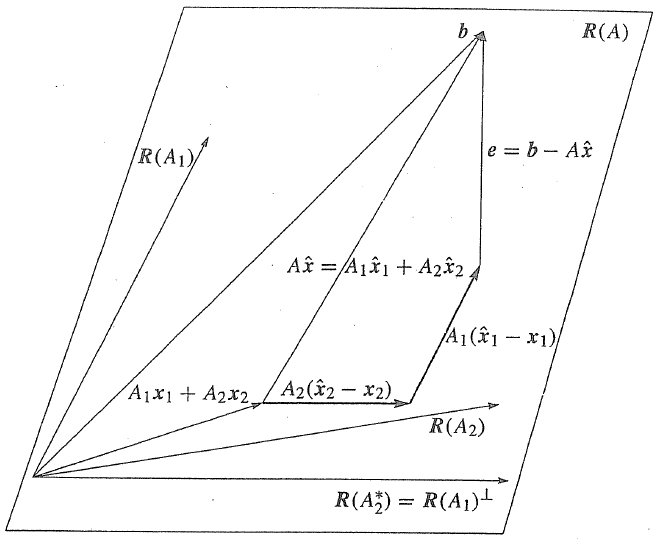
\includegraphics[width=0.7\linewidth]{TeX_files/Part02/chapter06/image/6-3}
	\caption{ $A=[A1 \ A2]$  中A的列空间中正交分解的几何图形}
\end{figure}

\subsection{观测方程的消元}

如果我们直接对观测方程使用上述过程是可以求解的,但是我们通常得到错误的结果。列空间必须被分成符合将$A$分割成$[A1 A2]$的两个子空间,此外,两个子空间必须是正交。

首先,将观测方程划分为
\begin{align}
\begin{bmatrix}
A_{1}\\
A_{2}
\end{bmatrix}
\begin{bmatrix}
\textbf{\textit{x}}_{1} & \textbf{\textit{x}}_{2}
\end{bmatrix} = \textbf{\textit{b}}.
\end{align}
$A =[A1 A2]$的列空间$R(A)$。我们将$R(A)$分解为$A_{1}$列空间和其正交补间$\textbf{R}^{\bot} $所覆盖的空间$\textbf{R}(A_{1})$。根据定义,我们有$ A^{T}_{1}CA^{*}_{2} = 0 $其中$ A^{*}_{2}$ 跨越 $\textbf{R}^{\bot} $。

投影$P = I -A_{1}(A^{T}_{1}CA_{1})^{-1}A^{T}_{1}C $将$\textbf{R}(A)$中的$A_{2}$投影至$\textbf{R}^{\bot} $中的$ A^{*}_{2}$
\begin{align*}
A^{*}_{2} = (I -A_{1}(A^{T}_{1}CA_{1})^{-1}A^{T}_{1}C)A_{2}.
\end{align*}
减少的观测方程是
\begin{align*}
(I -A_{1}(A^{T}_{1}CA_{1})^{-1}A^{T}_{1}C)A_{2}\textbf{\textit{x}}_{2} =
(I -A_{1}(A^{T}_{1}CA_{1})^{-1}A^{T}_{1}C)\textbf{\textit{b}}
\end{align*}
或缩写
\begin{align*}
A^{*}_{2}\textbf{\textit{x}}_{2} = \textbf{\textit{b}}^{*}.
\end{align*}
接下来我们解决$ \textbf{\textit{x}}_{2}$:
\begin{align}
\textbf{\textit{x}}_{2} = ( A^{*^T}_{2}CA^{*}_{2} )^{-1}A^{*^T}_{2}C \textbf{\textit{b}}^{*}.
\end{align}
上述过程具有重要的应用。当处理$GPS$观测值时可能想要消除歧义未知数。我们重写(6.52)
\begin{align*}
A_{1}\textbf{\textit{x}}_{1} + A_{2}\textbf{\textit{x}}_{2} = \textbf{\textit{b}}.
\end{align*}
未知数$\textbf{\textit{x}}_{1}$通过乘以$\textbf{R}^{\bot}$的投影$\textbf{P}$去除:
\begin{align*}
PA_{1}\textbf{\textit{x}}_{1} + PA_{2}\textbf{\textit{x}}_{2} = P\textbf{\textit{b}}.
\end{align*}
当$PA_{1}=0$时,变换后的观测方程变为
\begin{align*}
A^{*}_{2}\textbf{\textit{x}}_{2}= \textbf{\textit{b}}^{*}.
\end{align*}
我们描述了图6.3中这种正交分解的几何形状。

最后,我们想要演示从(6.41)观察的程序。系数矩阵$A$被分成两列$[A1 A2]$。投影$P$变为
\begin{align*}
P = \dfrac{1}{4}
\begin{bmatrix}
3 & -1 & -1 & -1 \\
-1 & 3 & -1 & -1 \\
-1 & -1 & 3 & -1 \\
-1 & -1 & -1 & 3 
\end{bmatrix}.
\end{align*}
变换的观测方程为$A^{*}_{2}\textbf{\textit{x}}_{2} = \textbf{\textit{b}}^{*} $
\begin{align*}
\begin{bmatrix}
-2 \\
-1 \\
1 \\
2 
\end{bmatrix}
\textbf{\textit{x}}_{2}= 
\begin{bmatrix}
-9 \\
-1 \\
-1 \\
11 
\end{bmatrix}.
\end{align*}
方程为$10\hat{\textbf{\textit{x}}}_{2}=40$,解法再次恢复为$\hat{\textbf{\textit{x}}}_{2} = 4 $。

 错误计算运行如下:
 \begin{align*}
 \hat{\textbf{\textit{e}}} = \textbf{\textit{b}}^{*} -A^{*}_{2} \hat{\textbf{\textit{x}}}_{2} =
 \begin{bmatrix}
 -9 \\
 -1 \\
 -1 \\
 11 
 \end{bmatrix} -
 \begin{bmatrix}
 -2 \\
 -1 \\
 1 \\
 2 
 \end{bmatrix}4 = 
 \begin{bmatrix}
 -1 \\
 3 \\
 -5 \\
 3 
 \end{bmatrix};
 \end{align*}
 和
 \begin{align*}
 \hat{\sigma}^{2}_{0} = \dfrac{44}{4-2} = 22 .
 \end{align*} 
 该过程在$M$文件消除中编码。